\documentclass[a4paper,11pt]{ltjsarticle}
% 数式
\usepackage{amsmath,amsfonts}
\usepackage{bm}
% 画像
\usepackage{graphicx}
\usepackage{circuitikz}
\usepackage{amsmath,amssymb}
\usepackage{siunitx}
\usepackage{float}
\usepackage{tikz}
\usepackage{askmaps}
\usepackage{multirow}
\usepackage{bigstrut}
\usepackage{slashbox}
\usepackage{rotating}
\usepackage{listings}
% 数式
\usepackage{physics}
\usepackage{mathtools}
% 画像
\usepackage{subcaption}
% 表
\usepackage{makecell}
% その他
\usepackage{url}
\usepackage{ascmac}
\usepackage{cases}
\usepackage{here}
\usepackage{upgreek}
% 日本語対応
\usepackage{luatexja}
\usepackage{luatexja-fontspec}

\AtBeginDocument{\RenewCommandCopy\qty\SI}


% \definecolor{commentgreen}{RGB}{0,200,0}
% \definecolor{eminence}{RGB}{120,80,250}
% \definecolor{weborange}{RGB}{255,165,0}
% \definecolor{frenchplum}{RGB}{10,150,200}
% \definecolor{commentgreen}{RGB}{0,200,0}
% \definecolor{eminence}{RGB}{120,80,250}
% \definecolor{weborange}{RGB}{255,165,0}
% \definecolor{frenchplum}{RGB}{10,150,200}

\lstset{
        language = {C},
        basicstyle = \ttfamily\small,
        % keywordstyle=\color{eminence}\ttfamily\bfseries,
        % commentstyle=\color{commentgreen}\textit,
    % identifierstyle=\color{black}\ttfamily,
        xleftmargin=.35in,
        frame=lines,
    showstringspaces=false,
        numbers=left,
        stepnumber = 1,
        breaklines=true,
        numberstyle = \ttfamily\normalsize,
    tabsize=4,  
        emph={int, int8_t, int16_t, int32_t, int64_t, uint8_t, uint16_t, uint32_t, uint64_t, char, double, float, unsigned, void, bool},
        % emphstyle={\color{blue}}, 
        morekeywords={>, <, ., ;, +, -, *, /, !, =, ~},
        breakindent = 10pt, 
        framexleftmargin=10mm, 
        columns=fixed,
        basewidth=0.5em,
        }

% 特定のスタイル設定
\lstdefinestyle{customtxt}{
  basicstyle=\ttfamily\footnotesize,
  backgroundcolor=\color{lightgray},
  frame=single,
  breaklines=true,
  columns=fullflexible,
  showspaces=false,
  showstringspaces=false,
  showtabs=false,
  tabsize=4,
}

\newcommand{\fig}[4]{
    \begin{figure}[htbp]
      \centering
      \includegraphics{./image/#1}
      \caption{#2}
      \label{fig:#3}
    \end{figure}
  }
\begin{document}
\section{目的}
本実験では，順序回路(10進数カウンタ)をHDLで設計し，シュミレーションを行い，
階層設計を行ってからモジュールごとの設計を行うことにより，
FPGAにおいて大規模な回路構築する手法を学ぶこと，そして
シュミレーションを行うことによりデバッグ作業を簡単化する方法について学ぶ．
また，学んだ手法を活かして，課題より拡張させた機能の実装を行う．
\section{原理}
本実験で使用するGPGA，HDL，Verilogについて説明する．
\subsection{階層設計}
大規模な回路を設計する際に，回路全体をモジュール単位に分割させ，
モジュールごとのつながりをブロック図として表現する．
各モジュールごとでの入出力を設計することにより，複雑な回路を簡単に設計することができる．
また，モジュールの内部は階層構造に関係ないため，モジュールごとに独立して設計を行うことができる．
\subsection{同期/非同期}
同期回路とは，クロック信号に同期して動作する回路であり，
クロックの立ち上がり/立下りに合わせて動作を行う．
一方非同期とはクロックに依存しない回路であり，
入力信号の立ち上がり/立下りに応じて動作を行う．
\subsection{分周器}
分周器とは，入力信号に対して一定の比率で出力信号を生成する回路である．
クロック信号に同期したカウンタ回路とマジックナンバー(今回は分周する比率)を比較し，
所定のカウント数に達したときに出力信号を切り替えることにより，分周を実現する．
\subsection{ダイナミック点灯}
7セグメントの表示回路では，FPGAから出力電流($8m[A]$)を増幅させ，LEDを明るくするためにソーストランジスタが用いられている．
これらは一つのLEDに対して一つのトランジスタ(実際にはダーリントントランジスター構成になっていたり，
クランプ回路が挟まっている)を配置しているため，本実験で使用するFPGAボードでは8chの
ソーストランジスタアレイを用いている．これにより，$8m[A]$を$20m[A]$に増幅させている．
これらの回路を4桁分用意すると，必要なICの数が4個となり，回路がでかくなってしまう．
そこでダイナミック点灯を用いる．
7セグメントLEDのコモンカソード側にシンクトランジスタアレイを配置している．これにより，
各桁のコモンカソード側をGNDにした桁にのみソーストランジスタアレイからの電流が流れる．
この構成ではソーストランジスタアレイの各出力が4つの7セグメントLEDのピンと同じように配線されている．
そのため，ソーストランジスタアレイの入力とシンクトランジスタアレイの入力を同期させることにより，高速で桁の切り替えを行うことが出来る．
人間の目では一定値以上の速度の切り替えを行うと同時に点滅しているように見える(残像効果)ため，
4桁分の7セグメントLEDを少ないICで点灯させることが出来る．
\section{実験環境}
表\ref{tab:zikken}に使用するソフトウェアとハードウェアについての実験環境を示す．
\begin{table}[H]
    \centering
    \caption{実験環境}
    \label{tab:zikken}
    \begin{tabular}{|c|c|}
        \hline
        項目             & 内容                                   \\
        \hline
        FPGAボード        & Gowin社製 GW1NR-9                      \\
        \hline
        開発ソフトウェア       & Gowin\_V1.9.11.03 Education (64-bit) \\
        \hline
        シミュレーションソフトウェア & iverilog                             \\
        \hline
    \end{tabular}
\end{table}
\section{実験方法}
本実験で行った実験手順を示す．また，課題に対して追加した機能についても記載する．
\subsection{ブロック図(階層設計)}
本実験で作成するものについて，仕様を決めてからブロック図を作成し，
モジュール間の接続を明確にする．また，それぞれのモジュールについての動作についても仕様を決める．
\subsection{HDLの作成}
ブロック図をもとにHDLを作成する．本実験ではVerilogを用いてHDLを作成する．
\subsection{シミュレーション}
作成したHDLが正しく動作するかをテストベンチを作成し，シミュレーションを行い確認する．
\subsection{FPGAへの書き込み}
シミュレーションで正しく動作することが確認できたら，FPGAボードに書き込みを行い，シュミレーションと同じ動きをするか確認する．
\subsection{動作確認}
FPGAボードに書き込みを行った後，実際に動作確認を行う．
\section{結果}
実験方法を参照し，実験を行った．
\subsection{ブロック図}
図\ref{fig:block}に全加算器/全減算機の組み合わせ回路のブロック図を示す．
また，各モジュールの仕様について示す(トップモジュールから見た動作仕様であり，
内部の動作については実装した後に後述する)．
\newpage
\begin{figure}[H]
    \centering
    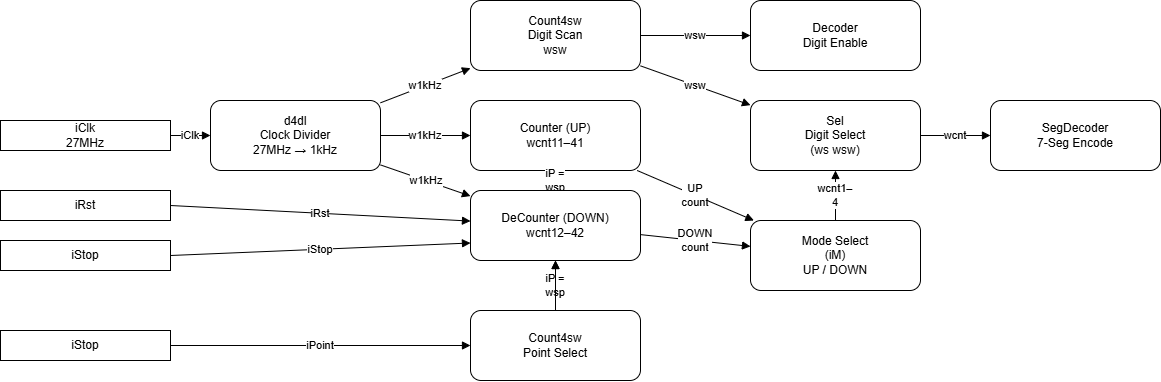
\includegraphics[width=1.4\linewidth,angle=90]{./image/block_logical.drawio.png}
    \caption{全加算器/全減算機の組み合わせ回路のブロック図}
    \label{fig:block}
\end{figure}
\newpage
\subsubsection{分周器(d4dl)}
d4dl(DividerForDynamicLighting)は，
システムクロックの27$m[\text{Hz}]$を1$k[\text{Hz}]$に分周する回路である．
ダイナミック点灯と，7桁の10進カウンタの動作に使用している．
入出力のピンの仕様を表\ref{tab:d4dl}に示す．
\begin{table}[H]
    \centering
    \caption{分周器(d4dl)の入出力ピン仕様}
    \label{tab:d4dl}
    \begin{tabular}{|c|c|c|}
        \hline
        ピン名  & 種類 & 説明       \\
        \hline
        iClk & 入力 & システムクロック \\
        \hline
        oClk & 出力 & 分周後クロック  \\
        \hline
    \end{tabular}
\end{table}
\subsubsection{4進カウンタ(Count4sw)}
Count4sw(Count4switch)は，入力に応じて0から3までの4進カウントを行う回路である．
今回は二個用いている．
これは小数点表現をするために使用しており，
1$k[\text{Hz}]$のクロック信号よりダイナミック点灯させている回路を制御しているため，
今表示させている桁をwswの信号で保持している．
また，もう一つの回路では，スイッチの入力により4進カウンタを動作させており，
小数点の位置を記憶している．小数点の位置とwspの対応表を表\ref{tab:wsw}に示す．
入出力のピンの仕様を表\ref{tab:count4sw}に示す．
\begin{table}[H]
    \centering
    \caption{小数点位置とwswの対応表}
    \label{tab:wsw}
    \begin{tabular}{|c|c|}
        \hline
        wswの値 & 小数点位置 \\
        \hline
        00    & 0桁目   \\
        \hline
        01    & 1桁目   \\
        \hline
        10    & 2桁目   \\
        \hline
        11    & 3桁目   \\
        \hline
    \end{tabular}
\end{table}
\begin{table}[H]
    \centering
    \caption{4進カウンタ(Count4sw)の入出力ピン仕様}
    \label{tab:count4sw}
    \begin{tabular}{|c|c|c|}
        \hline
        ピン名  & 種類 & 説明      \\
        \hline
        iClk & 入力 & クロック信号  \\
        \hline
        oSw  & 出力 & 4進カウント値 \\
        \hline
    \end{tabular}
\end{table}
\subsubsection{7桁の10進カウンタ(Counter/DeCounter)}
Counter/DeCounterは，7桁の10進カウンタである．
Counterはカウントアップ，DeCounterはカウントダウンを行う．
wspの信号による小数点位置により，7桁のカウンタの値を1桁目，2桁目，3桁目，4桁目の出力とのつながりを変えている．
入出力のピンの仕様を表\ref{tab:counter}に示す．
\begin{table}[H]
    \centering
    \caption{7桁の10進カウンタ(Counter/DeCounter)の入出力ピン仕様}
    \label{tab:counter}
    \begin{tabular}{|c|c|c|}
        \hline
        ピン名   & 種類 & 説明        \\
        \hline
        iClk  & 入力 & クロック信号    \\
        \hline
        iRst  & 入力 & リセット信号    \\
        \hline
        iStop & 入力 & カウント停止信号  \\
        \hline
        iP    & 入力 & 小数点位置保持信号 \\
        \hline
        oCnt1 & 出力 & 1桁目カウント値  \\
        \hline
        oCnt2 & 出力 & 2桁目カウント値  \\
        \hline
        oCnt3 & 出力 & 3桁目カウント値  \\
        \hline
        oCnt4 & 出力 & 4桁目カウント値  \\
        \hline
    \end{tabular}
\end{table}
\subsubsection{4入力マルチプレクサ(Sel)}
Sel(Selector)は，4入力マルチプレクサである．
ダイナミック点灯を行うために，4桁の出力をwswの信号により選択している．
これにより，今表示している桁の値をソーストランジスタアレイの入力として出力している．
入出力のピンの仕様を表\ref{tab:sel}に示す．
\begin{table}[H]
    \centering
    \caption{4入力マルチプレクサ(Sel)の入出力ピン仕様}
    \label{tab:sel}
    \begin{tabular}{|c|c|c|}
        \hline
        ピン名  & 種類 & 説明        \\
        \hline
        iA   & 入力 & 1桁目に表示する値 \\
        \hline
        iB   & 入力 & 2桁目に表示する値 \\
        \hline
        iC   & 入力 & 3桁目に表示する値 \\
        \hline
        iD   & 入力 & 4桁目に表示する値 \\
        \hline
        iSw  & 入力 & 小数点位置保持信号 \\
        \hline
        oOut & 出力 & 選択された値    \\
        \hline
    \end{tabular}
\end{table}
\subsubsection{7セグメント用デコーダ(SegDecoder)}
SegDecoder(SegmentDecoder)は，7セグメントLED表示用のデコーダーである．
4bitの2進数を7セグメントLEDの点灯パターンに変換する回路である．
入出力のピンの仕様を表\ref{tab:segdecoder}に示す．
\begin{table}[H]
    \centering
    \caption{4出力デコーダ―(SegDecoder)の入出力ピン仕様}
    \label{tab:segdecoder}
    \begin{tabular}{|c|c|c|}
        \hline
        ピン名 & 種類 & 説明                     \\
        \hline
        iD  & 入力 & デコードする前の2進数(4bit)      \\
        \hline
        iS  & 入力 & 小数点を表示するかの信号(1bit)     \\
        \hline
        oD  & 出力 & 7セグメントLEDの点灯パターン(8bit) \\
        \hline
    \end{tabular}
\end{table}
\subsubsection{4出力デコーダ―(Decoder)}
Decoderは，2bitの2進数を4bitの1hot信号(1つのbitだけ1であり，他のBitは0の信号)
に変換する回路である．これによりダイナミック点灯のシンクトランジスタアレイに入力する信号を生成している．
入出力のピンの仕様を表\ref{tab:decoder}に示す．
\begin{table}[H]
    \centering
    \caption{4出力デコーダ―(Decoder)の入出力ピン仕様}
    \label{tab:decoder}
    \begin{tabular}{|c|c|c|}
        \hline
        ピン名 & 種類 & 説明                \\
        \hline
        iA  & 入力 & デコードする前の2進数(2bit) \\
        \hline
        oF  & 出力 & 1hot信号(4bit)      \\
        \hline
    \end{tabular}
\end{table}
\subsection{HDLの作成}
トップモジュールから見た動作仕様に基づき，各モジュールのHDLを作成した．
各モジュールのプログラムとその説明を以下に示す．
\subsubsection{分周器(d4dl)}
分周器(d4dl)のHDLコードをリスト\ref{lst:d4dl}に示す．
動作て順としては，内部のレジスタでクロックの立ち上がりをカウントし，
所定(13499)のカウント数に達したときに出力クロックを反転させ，レジスタをクリアする．
このマジックナンバーは，以下の式で求めることが出来る．2で割っている理由としては，立ち上がりクロックのみで立ち上がりと立下りを出力させているためである(反転動作を行うため)．
また，-1している理由としては，0でリセットを行っているため，1からではなく0からカウントをするためである．

\begin{align}
    \frac{\text{入力クロック周波数}[\text{Hz}]}{\text{出力クロック周波数}[\text{Hz}]} - 1 & = \text{マジックナンバー} \\
    \frac{27[\text{MHz}]}{2 \times 1[\text{kHz}]} - 1                   & = 13499
\end{align}
\newpage
\lstinputlisting[caption=分周器(d4dl)のHDLコード,label=lst:d4dl,firstline=19,lastline=34]{./prog/divider.v}
\subsubsection{4進カウンタ(Count4sw)}
4進カウンタ(Count4sw)のHDLコードをリスト\ref{lst:count4sw}に示す．
このプログラムでは，内部のレジスタをそのまま出力に使ったコードで，
内部レジスタの値が$(3)_{10}$になったときに内部レジスタの値を$(0)_{10}$をすることにより，
簡単な4進カウンタを実現している．
\lstinputlisting[caption=4進カウンタ(Count4sw)のHDLコード,label=lst:count4sw,firstline=207,lastline=219]{./prog/Counter100.v}
\subsubsection{7桁の10進カウンタ(Counter/DeCounter)}
7桁の10進カウンタ(Counter/DeCounter)のHDLコードをリスト\ref{lst:counter}に示す．
このプログラムでは7つの内部レジスタをそれぞれカウントアップさせるコードであり，クロックに同期している．
iRstが0の場合，すべての桁を0にし(同期リセット)，またiStopが1のときにすべての桁のカウントアップを一時的に停止させるコードとなっている．
iRstが0かつ，iStopが1のときには，内部のカウンタ回路が動作するようになっている．
内部のカウンタでは，一番下の桁がクロック信号の立ち上がりと同期してカウントアップし，
各桁が$(10)_{10}$になったときに次の桁をひとつカウントアップさせ，その桁は$(0)_{10}$にリセットする動作を行っている．
これにより，7桁の10進カウンタを実現している．
また，wspの信号により，小数点位置に応じて各桁の出力を入れ替える動作を行っている．
\lstinputlisting[caption=7桁の10進カウンタ(Counter/DeCounter)のHDLコード,label=lst:counter,firstline=1,lastline=205]{./prog/Counter100.v}
\subsubsection{4入力マルチプレクサ(Sel)}
4入力マルチプレクサ(Sel)のHDLコードをリスト\ref{lst:sel}に示す．
このプログラムでは，入力された4つの信号の中から，iSwの信号に応じて1つを選択して出力するコードとなっている．
Self関数において，case文を用いて，oOutと入力された信号のつながりを変更している．
\newpage
\lstinputlisting[caption=4入力マルチプレクサ(Sel)のHDLコード,label=lst:sel,firstline=1,lastline=25]{./prog/Selector.v}
\subsubsection{7セグメント用デコーダ(SegDecoder)}
7セグメント用デコーダ(SegDecoder)のHDLコードをリスト\ref{lst:segdecoder}に示す．
このプログラムでは，入力された4bitの2進数を7セグメントLEDの点灯パターンに変換するコードとなっている．
また，iSの信号が1のときに小数点を点灯させる動作を行っている．
\lstinputlisting[caption=7セグメント用デコーダ(SegDecoder)のHDLコード,label=lst:segdecoder,firstline=1,lastline=25]{./prog/Decoder.v}
\subsubsection{4出力デコーダ―(Decoder)}
4出力デコーダ―(Decoder)のHDLコードをリスト\ref{lst:decoder}に示す．
このプログラムでは，入力された2bitの2進数を4bitの1hot信号に変換するコードとなっている．
\lstinputlisting[caption=4出力デコーダ―(Decoder)のHDLコード,label=lst:decoder,firstline=27,lastline=44]{./prog/Decoder.v}
\subsection{トップモジュール(MAIN)}
トップモジュール(MAIN)のHDLコードをリスト\ref{lst:main}に示す．
このプログラムでは，各モジュールをインスタンス化し，接続を行っている．
また，トップモジュールでは，全加算器/全減算機の組み合わせ回路の動作仕様に基づき，
スイッチの入力によりカウントアップ/カウントダウンの切り替えを行っている．
\lstinputlisting[caption=トップモジュール(MAIN)のHDLコード,label=lst:main,firstline=1,lastline=49]{./prog/main.v}
\subsection{シミュレーション}
作成したHDLが正しく動作するかをテストベンチを作成し，シミュレーションを行い確認した．
今回のコードでは初期状態では，w1kHzのクロック信号が1k回分立ち上がった後に，
最初の桁が繰り上がりされる．また，w1kHzもiClkを13500回分立ち上がった後に出力が反転する．そのためsimulationに非常に時間がかかるため，
最初にiPointの信号を(11)に設定し，小数点位置を3桁目に固定している．
また，すべてのモジュールのクロック入力でw1kHzを使用しているところはiClkに置き換えてテストベンチを動作させた．
そして，加算/減算を行えるため，二種類の結果を示す．
加算の結果をシミュレーション1，減算の結果をシミュレーション2として示す．
テストベンチとして作成したコードをリスト\ref{lst:testbench}に示す．
\lstinputlisting[caption=全加算器/全減算機の組み合わせ回路のテストベンチコード,label=lst:testbench]{./prog/tb.v}
シミュレーション1の結果を図\ref{fig:sim1}に示す．
シミュレーション2の結果を図\ref{fig:sim2}に示す．
また，このシミュレーション結果にはテストベンチの下にあるトップモジュールの信号，wcnt1~4を含めており，10進数の可読性をあげている．
そしてこの実験結果の波形解析を以下で行う．
\subsubsection{シミュレーション1}
シミュレーション1では，加算動作を行うテストベンチであり，iStopが1になった次のクロックの立ち上がりで
wcnt1 = 1になることから，カウントアップが開始されていることが読める．
そして，iClkと同期して1ずつカウントアップされ，9の次に0になり，wcnt2が1になることから桁上がりもうまくいっていることがわかる．
次に，oD1~4とoDの出力を比べると，iStopが1になった次のクロックから10クロックまでの間，oD1=1ではないときoDは0を表しており，
oD1=1のときにoDはwcnt1の値を7セグメントLED用にデコードした値を示しているはずである．出力結果を確認すると，
wcnt1が3のとき，oD1が1のため確認をしてみると，oDは7セグメントLED用にデコードされた値である$(0b01001111)_2$を示しており，正しい動作をしていることがわかる．
よって，加算動作においての桁上がりと，7セグメントLED用のデコードが正しく動作していることが分かった．
\subsubsection{シミュレーション2}
シミュレーション2では，減算動作を行うテストベンチであり，iM = 1に設定されている．
シミュレーション1では7セグメントLED用のデコード回路が正しく動作することを確認できたため，カウントダウン動作のみを
確認する．
iStopが1になった次のクロックの立ち上がりでwcnt1 = 9になることから，カウントダウンが開始されていることが読める．
そして，iClkと同期して1ずつカウントダウンされ，0の次に9になり，wcnt2が8になることから桁下がりもうまくいっていることがわかる．
よって，減算動作においての桁下がりが正しく動作していることが分かった．
\newpage
\begin{figure}[H]
    \centering
    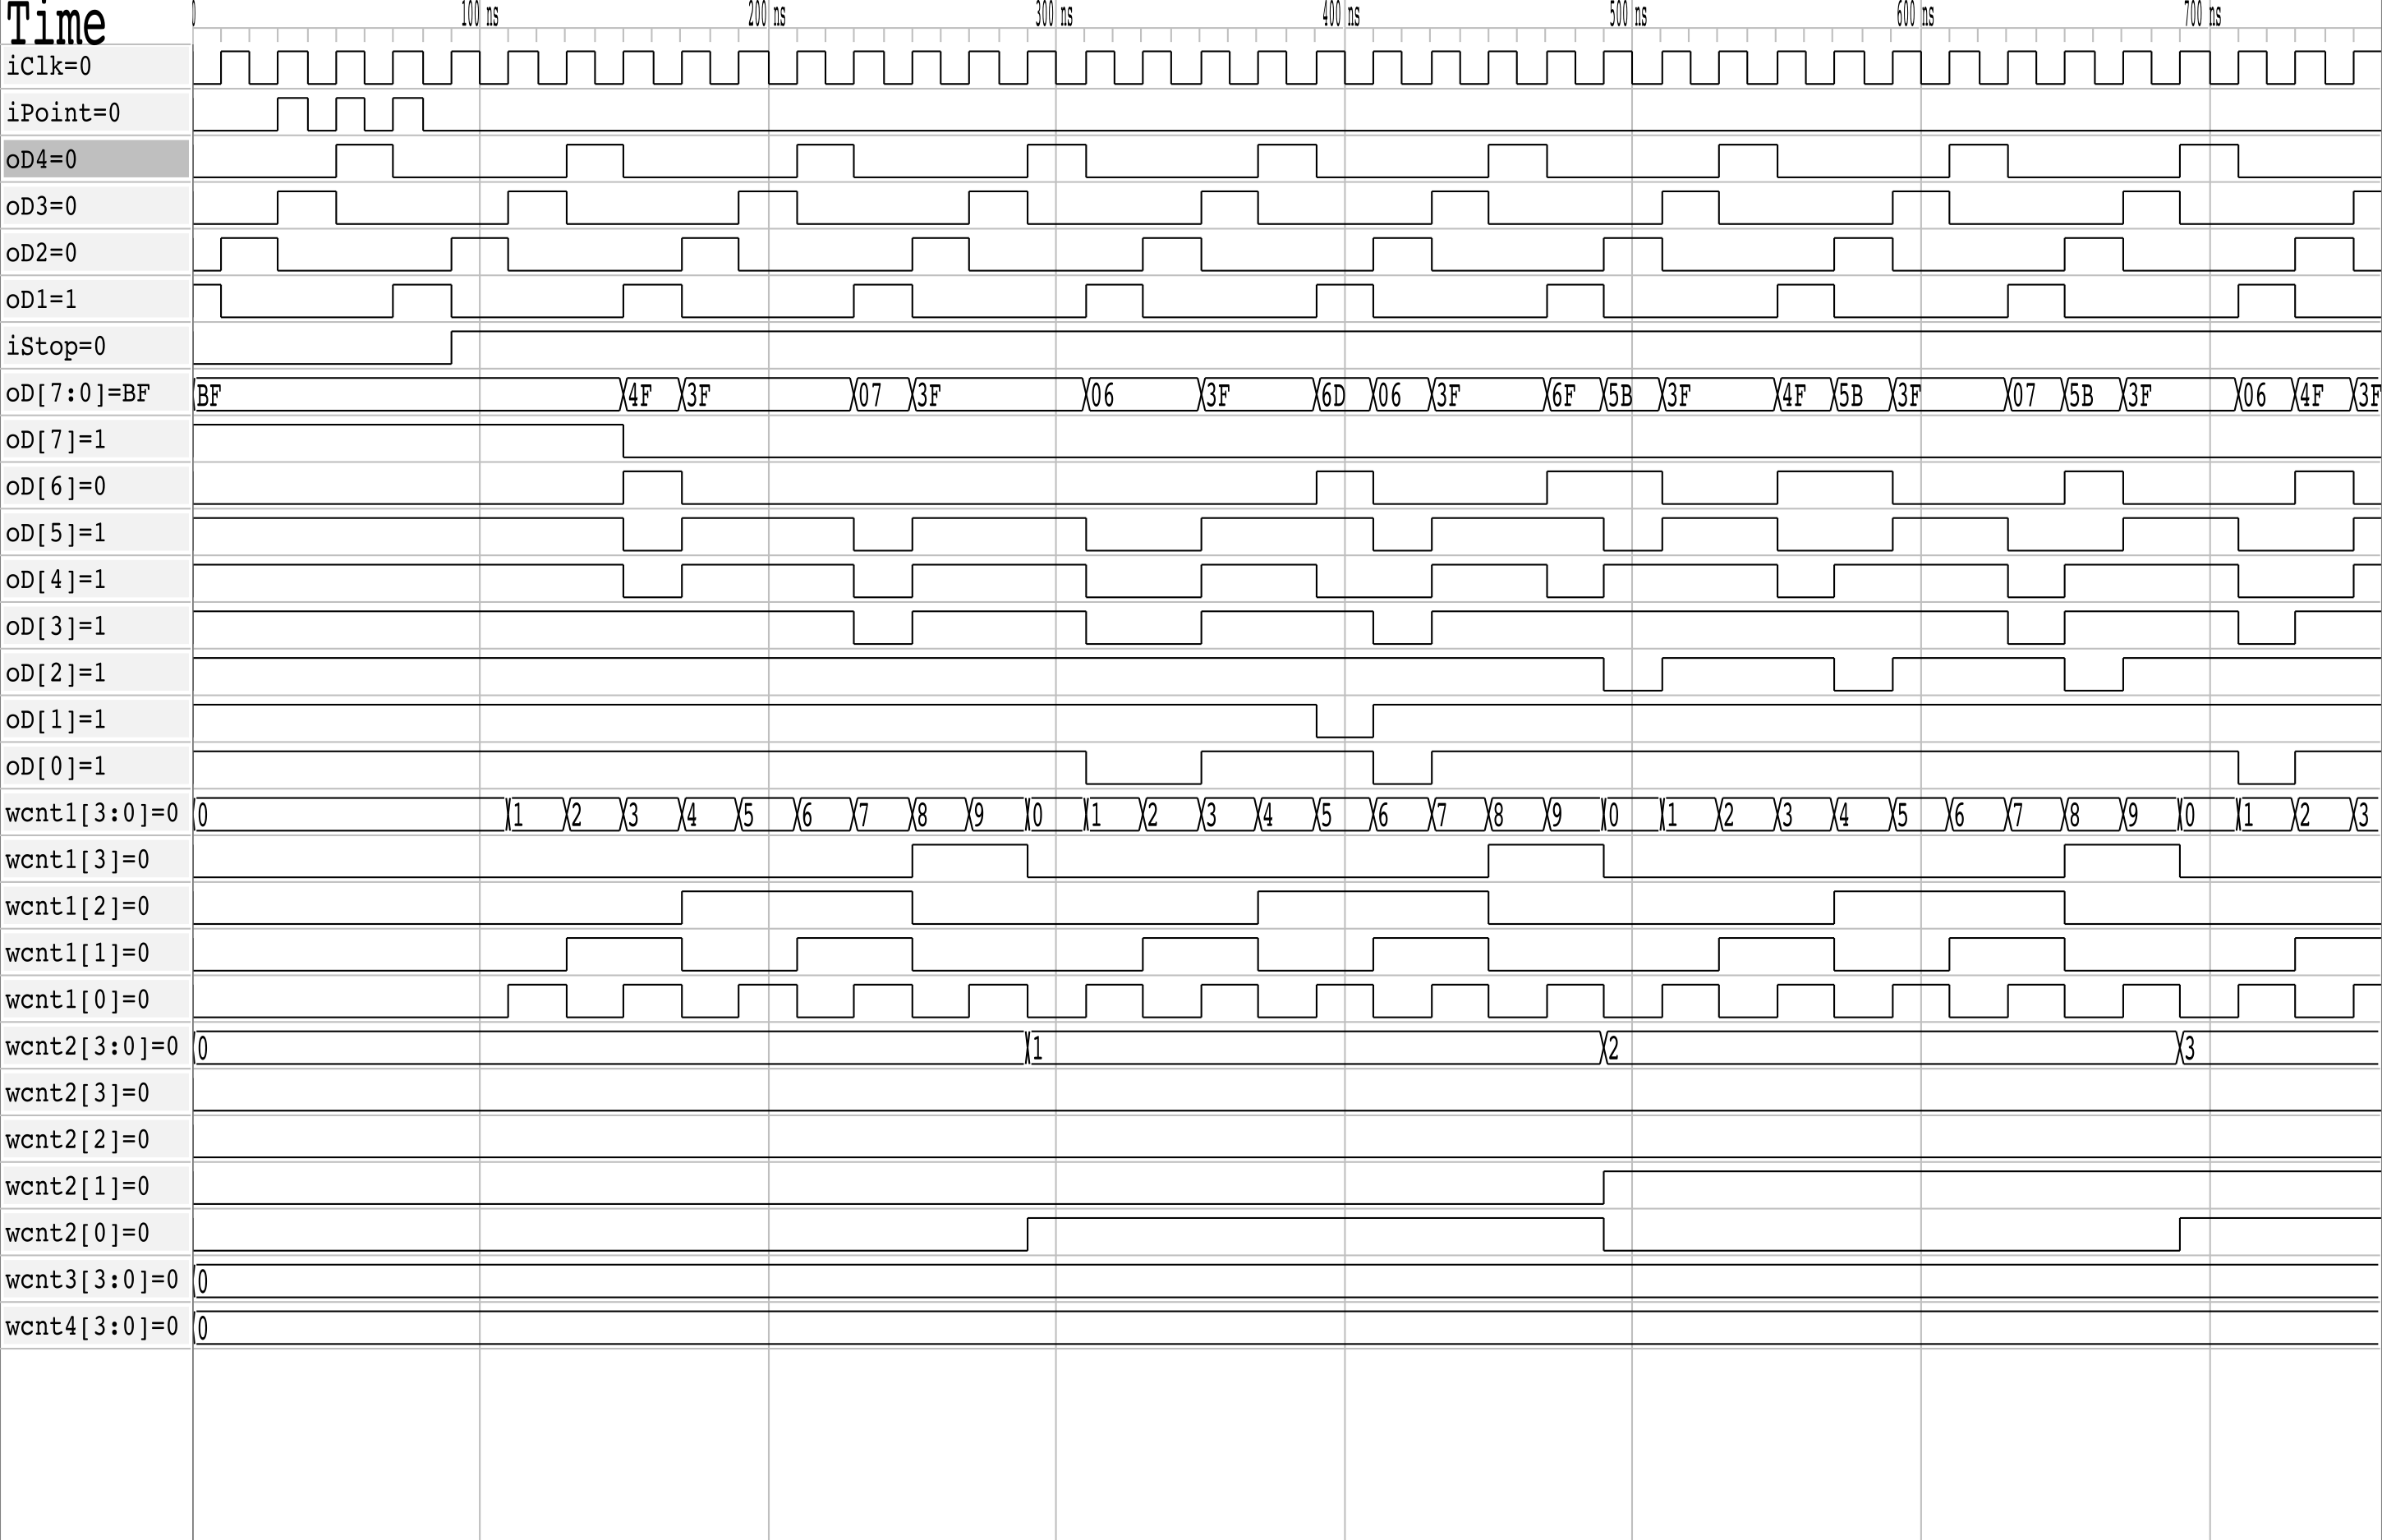
\includegraphics[width=1.4\linewidth,angle=90]{./image/sim2.png}
    \caption{シミュレーション結果1}
    \label{fig:sim1}
\end{figure}
\begin{figure}[H]
    \centering
    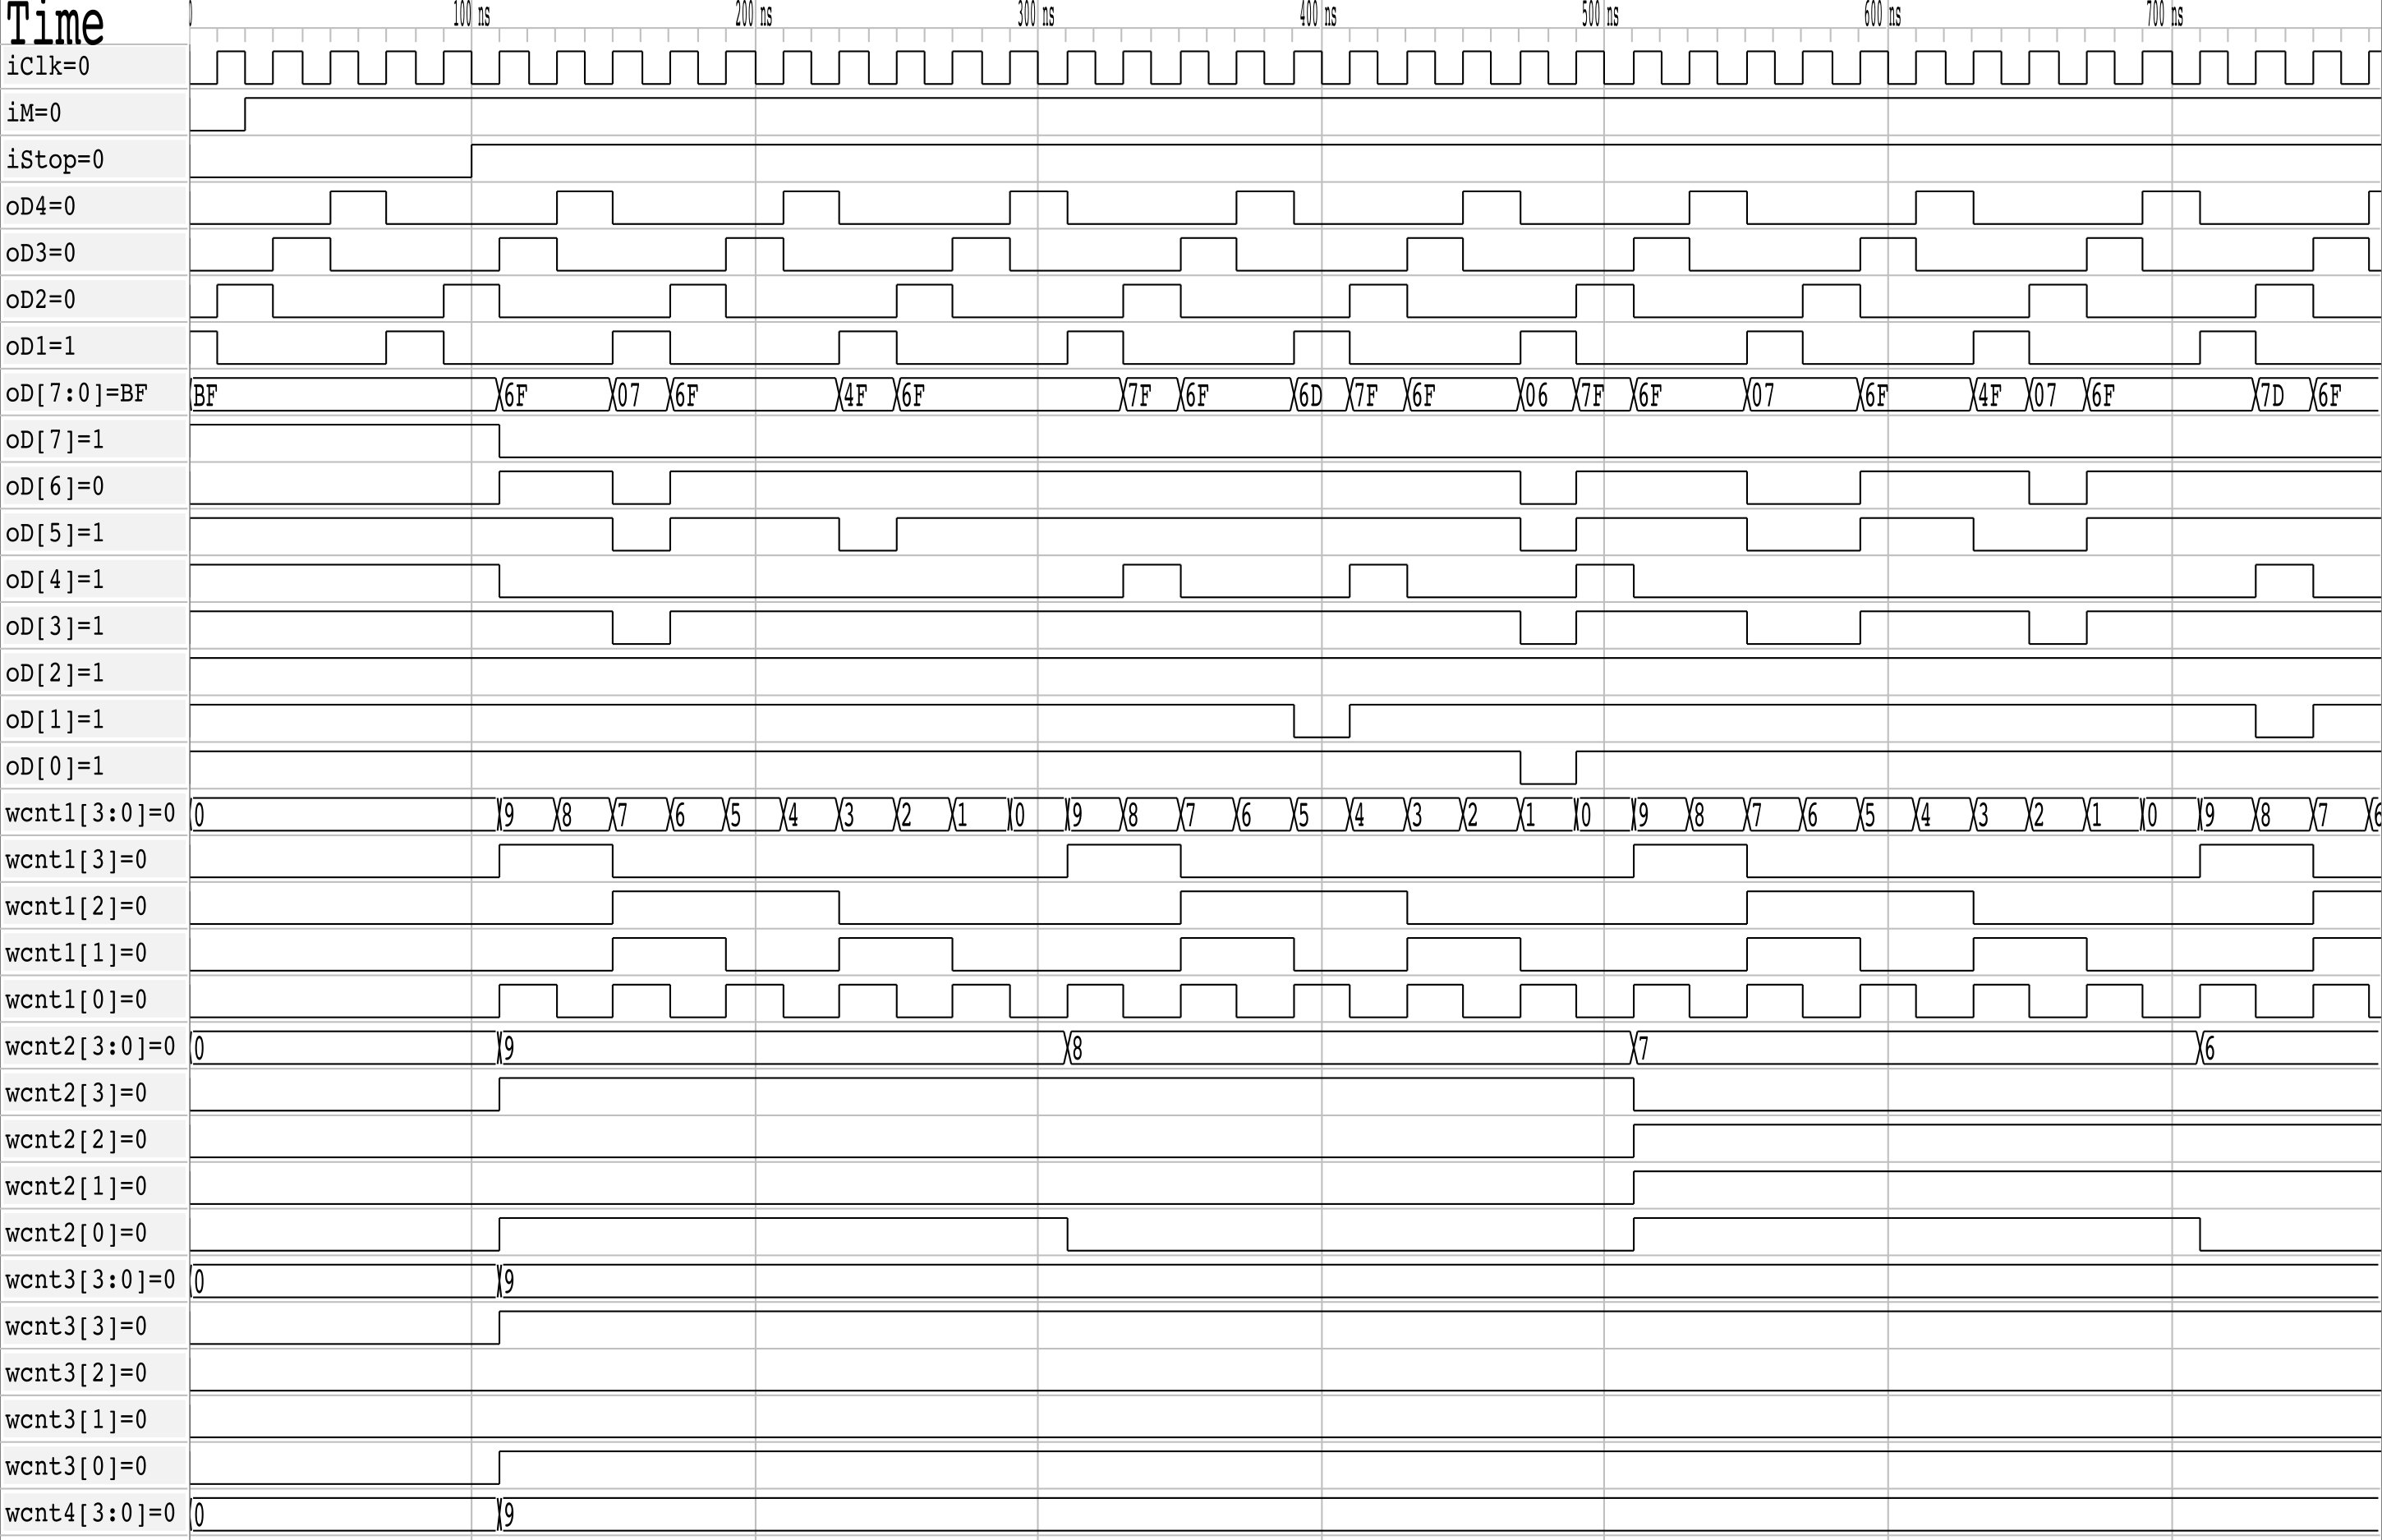
\includegraphics[width=1.4\linewidth,angle=90]{./image/sim3.png}
    \caption{シミュレーション結果2}
    \label{fig:sim2}
\end{figure}
\subsection{FPGAへの書き込み}
シミュレーションで正しく動作することが確認できたため，FPGAボードに書き込みを行った．
また，設定を行ったピン番号をリスト\ref{lst:pin}に示し，各信号との対応表を表\ref{tab:pin}に示す．
\begin{lstlisting}[caption=FPGAピン設定コード,label=lst:pin]
//Copyright (C)2014-2025 Gowin Semiconductor Corporation.
//All rights reserved. 
//File Title: Physical Constraints file
//Tool Version: V1.9.11.03 Education
//Part Number: GW1NR-LV9QN88PC6/I5
//Device: GW1NR-9
//Device Version: C
//Created Time: Wed 12 10 15:35:51 2025

IO_LOC "oD4" 86;
IO_PORT "oD4" IO_TYPE=LVCMOS18 PULL_MODE=UP DRIVE=8 BANK_VCCIO=1.8;
IO_LOC "oD3" 85;
IO_PORT "oD3" IO_TYPE=LVCMOS18 PULL_MODE=UP DRIVE=8 BANK_VCCIO=1.8;
IO_LOC "oD2" 84;
IO_PORT "oD2" IO_TYPE=LVCMOS18 PULL_MODE=NONE DRIVE=8 BANK_VCCIO=1.8;
IO_LOC "oD1" 83;
IO_PORT "oD1" IO_TYPE=LVCMOS18 PULL_MODE=NONE DRIVE=8 BANK_VCCIO=1.8;
IO_LOC "oD[7]" 49;
IO_PORT "oD[7]" IO_TYPE=LVCMOS18 PULL_MODE=NONE DRIVE=8 BANK_VCCIO=1.8;
IO_LOC "oD[6]" 48;
IO_PORT "oD[6]" IO_TYPE=LVCMOS18 PULL_MODE=NONE DRIVE=8 BANK_VCCIO=1.8;
IO_LOC "oD[5]" 70;
IO_PORT "oD[5]" IO_TYPE=LVCMOS18 PULL_MODE=NONE DRIVE=8 BANK_VCCIO=1.8;
IO_LOC "oD[4]" 71;
IO_PORT "oD[4]" IO_TYPE=LVCMOS18 PULL_MODE=NONE DRIVE=8 BANK_VCCIO=1.8;
IO_LOC "oD[3]" 72;
IO_PORT "oD[3]" IO_TYPE=LVCMOS18 PULL_MODE=NONE DRIVE=8 BANK_VCCIO=1.8;
IO_LOC "oD[2]" 73;
IO_PORT "oD[2]" IO_TYPE=LVCMOS18 PULL_MODE=NONE DRIVE=8 BANK_VCCIO=1.8;
IO_LOC "oD[1]" 74;
IO_PORT "oD[1]" IO_TYPE=LVCMOS18 PULL_MODE=NONE DRIVE=8 BANK_VCCIO=1.8;
IO_LOC "oD[0]" 75;
IO_PORT "oD[0]" IO_TYPE=LVCMOS18 PULL_MODE=NONE DRIVE=8 BANK_VCCIO=1.8;
IO_LOC "iRst" 4;
IO_PORT "iRst" IO_TYPE=LVCMOS18 PULL_MODE=NONE BANK_VCCIO=1.8;
IO_LOC "iStop" 3;
IO_PORT "iStop" IO_TYPE=LVCMOS18 PULL_MODE=UP BANK_VCCIO=1.8;
IO_LOC "iM" 31;
IO_PORT "iM" IO_TYPE=LVCMOS18 PULL_MODE=UP BANK_VCCIO=1.8;
IO_LOC "ipoint" 32;
IO_PORT "ipoint" IO_TYPE=LVCMOS18 PULL_MODE=UP BANK_VCCIO=1.8;
IO_LOC "iClk" 52;
IO_PORT "iClk" IO_TYPE=LVCMOS18 PULL_MODE=NONE BANK_VCCIO=1.8;

\end{lstlisting}
\begin{table}[H]
    \centering
    \caption{各信号との対応表}
    \label{tab:pin}
    \begin{tabular}{|c|c|c|c|}
        \hline
        信号名         & ピン番号 IOTYPE    & PULL MODE \\
        \hline
        oD4-oD1     & 83-86 LVCMOS18 & UP        \\
        \hline
        oD[7]-oD[0] & 49-75 LVCMOS18 & NONE      \\
        \hline
        iRst        & 4 LVCMOS18     & NONE      \\
        \hline
        iStop       & 3 LVCMOS18     & UP        \\
        \hline
        iM          & 31 LVCMOS18    & UP        \\
        \hline
        ipoint      & 32 LVCMOS18    & UP        \\
        \hline
        iClk        & 52 LVCMOS18    & NONE      \\
        \hline
    \end{tabular}
\end{table}
\subsection{動作確認}
FPGAボードに書き込みを行った後，実際に動作確認を行った．
画像\ref{fig:fpga1}では，露光時間を1/50秒に設定して撮影したものであり，ダイナミック点灯(1/1000秒)の4桁分の時間よりも長いためすべての桁がはっきり見れることを表している．
画像\ref{fig:fpga2}では，露光時間を1/6000秒に設定して撮影したものであり，ダイナミック点灯(1/1000秒)よりも短いため，1桁分しか見えないことを表している．
この二つの画像より，ダイナミック点灯が正しく動作していることが分かる．
また，操作機能として，iRstとiStop，また，iM，ipointのスイッチを操作することにより，
リセット，カウントの停止/再開，加算/減算，小数点位置の変更が正しく動作していることを確認した．
\begin{figure}[H]
    \centering
    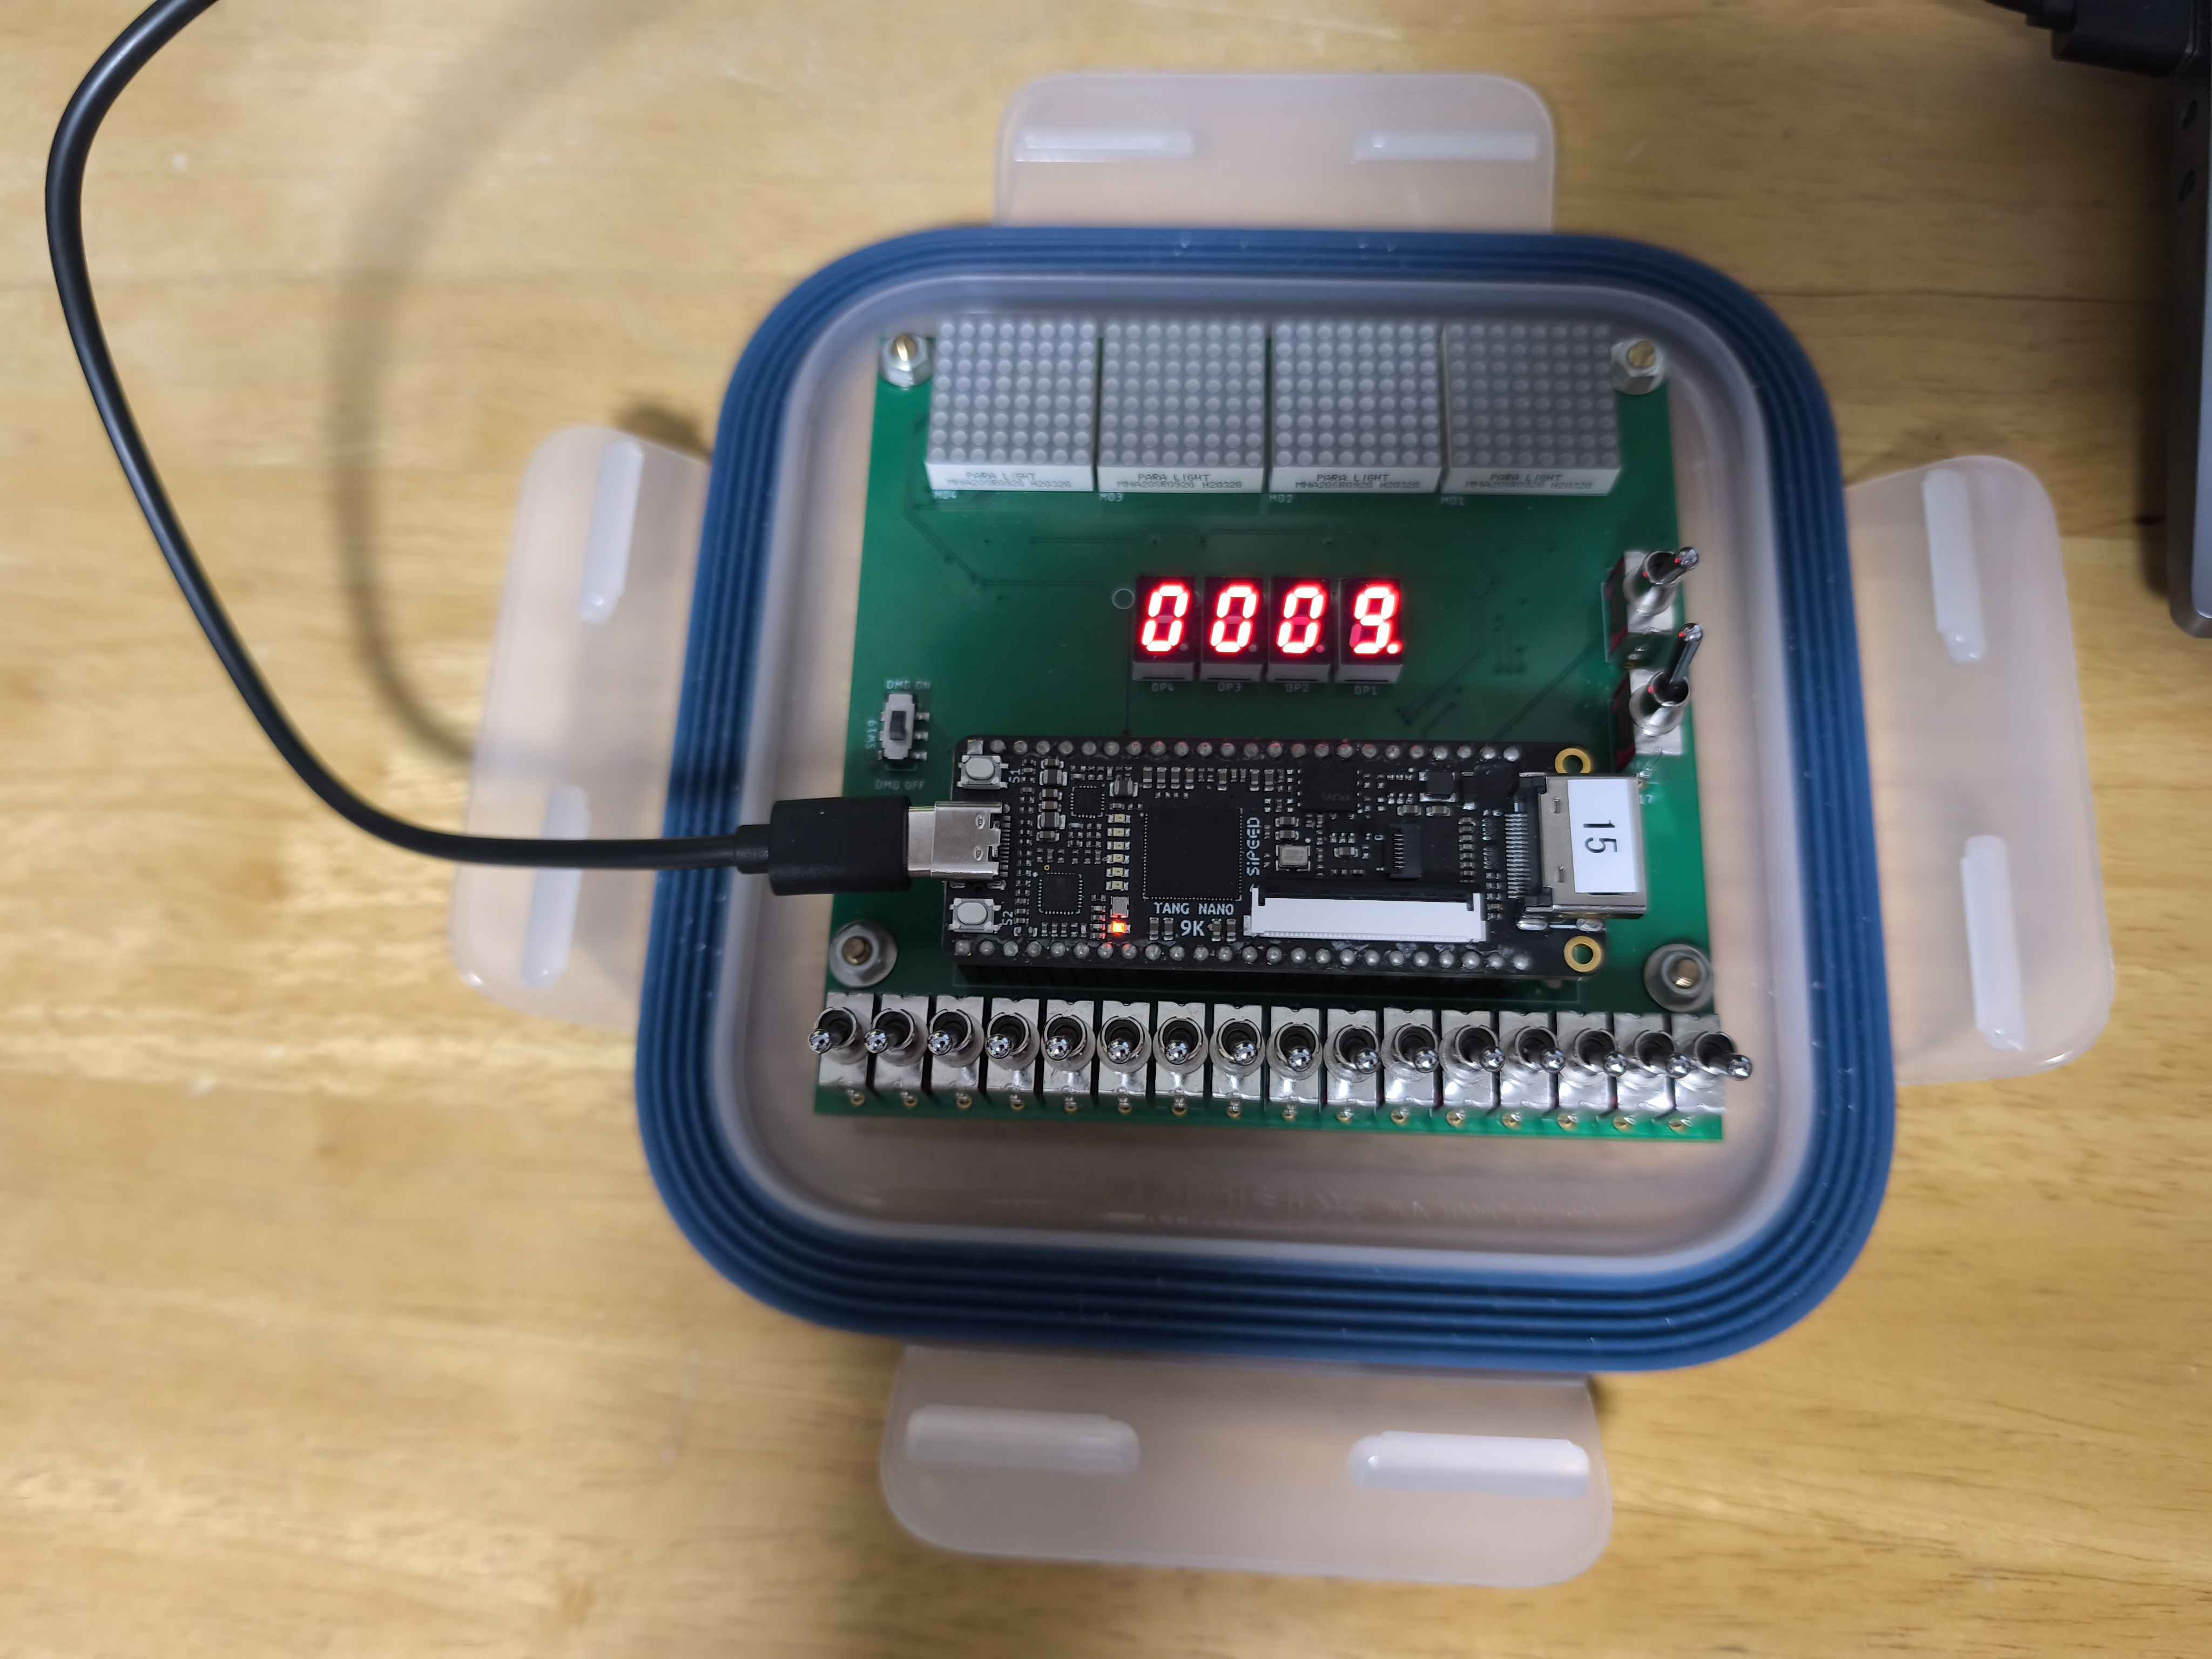
\includegraphics[width=0.6\linewidth]{./image/result1.jpg}
    \caption{FPGAボードの動作確認画像1(露光時間1/50秒)}
    \label{fig:fpga1}
\end{figure}
\begin{figure}[H]
    \centering
    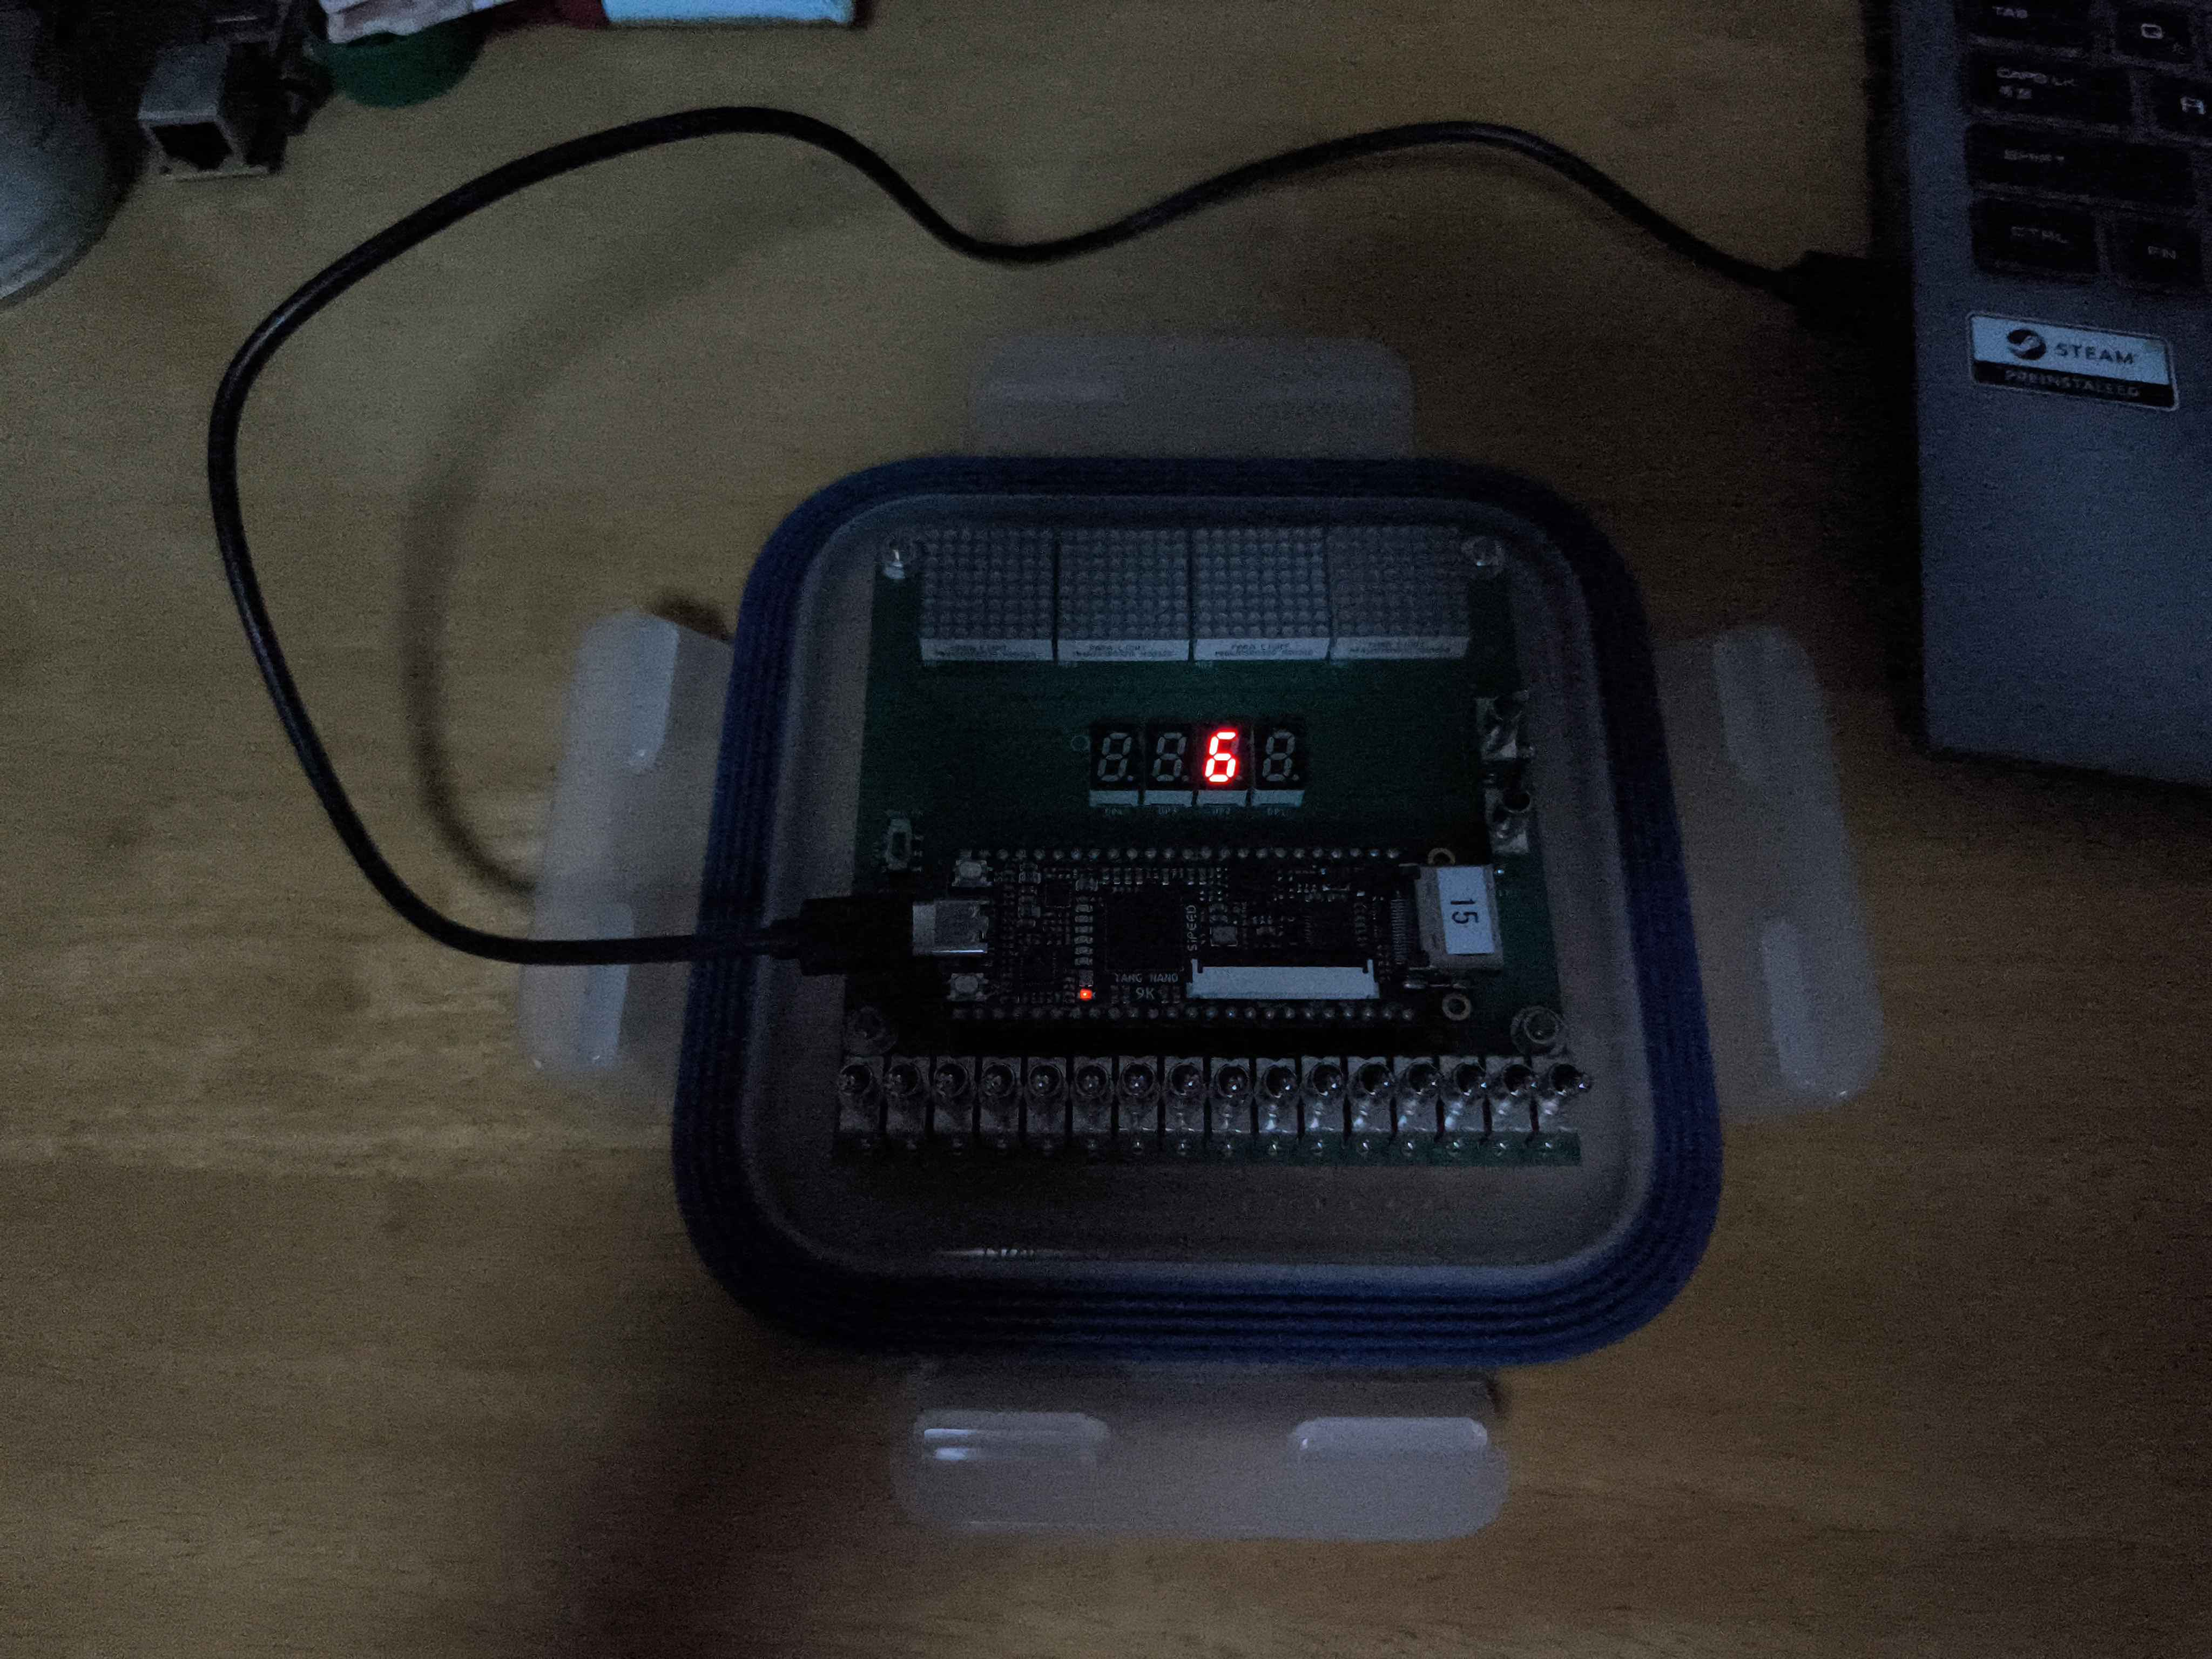
\includegraphics[width=0.6\linewidth]{./image/result2.jpg}
    \caption{FPGAボードの動作確認画像2(露光時間1/6000秒)}
    \label{fig:fpga2}
\end{figure}
\section{考察}
本実験で得られた結果をもとに，達成目標ごとの達成度と考察を述べる．
\subsection{順序回路の階層設計}
本実験では，順序回路(10進数カウンタ)をHDLで設計し，階層設計を用いて大規模な回路を構築する手法を実践した．
図\ref{fig:block}に示したブロック図のように，システム全体を分周器，カウンタ，セレクタ，デコーダといった
機能単位のモジュールに分割し，それぞれのモジュールに対して明確な入出力仕様を定義した．
この手法により，各モジュールの動作を独立して設計・検証することができ，
複雑な回路の実装を効率的に進めることができた．

特に，7桁の10進カウンタのように比較的複雑なモジュールにおいても，
入出力ピンの仕様を明確にすることで，トップモジュールでの配線が容易になり，
モジュール間の接続ミスを防ぐことができた．
また，各モジュールを独立して設計することで，デバッグ作業も効率化され，
問題が発生した際にも該当するモジュールに絞って原因を特定することが可能であった．

課題通りの設計を行った後に拡張機能を追加したため，
モジュールの命名規則や信号名の統一が重要であることも学んだ．
一貫した命名規則により，コードの可読性と保守性が向上し，
拡張時の混乱を防ぐことができた．

\subsection{HDL設計とシミュレーション}
Verilog HDLを用いた回路設計において，テストベンチを作成してシミュレーションを行うことの重要性を実感した．
特に本実験では，FPGAへの書き込み前にシミュレーションを行うことで，
カウンタの桁上がり・桁下がりの動作や，7セグメントLEDのデコード処理が正しく動作することを確認できた．

シミュレーション1では加算動作における桁上がりの動作を確認し，
wcnt1が9から0に変化する際にwcnt2が1増加することから，
正しく繰り上がり処理が行われていることが確認できた．
また，シミュレーション2では減算動作における桁下がりの動作を確認し，
wcnt1が0から9に変化する際にwcnt2が1減少することから，
正しく繰り下がり処理が行われていることが確認できた．

このように，シミュレーションを活用することで，
実機での動作確認前にロジックエラーを検出・修正することができ，
開発効率を大幅に向上させることができた．
シミュレーションによるデバッグ作業の簡単化という目的は十分に達成できたと言える．

\subsection{分周器の設計と動作}
システムクロック27MHzを1kHzに分周する回路を設計し，実装した．
分周比を決定するマジックナンバーの計算において，
出力クロックの反転動作を考慮して入力周波数を2倍で割る必要があることや，
0からカウントを開始するため-1する必要があることなど，
実装上の細かい注意点を理解することができた．

この分周器は，ダイナミック点灯とカウンタ動作の両方に使用されており，
システム全体の時間軸を制御する重要な役割を果たしている．
実際の動作確認でも安定して1kHzの信号が生成されており，
設計通りの動作が実現できたことを確認した．

\subsection{ダイナミック点灯の実装}
7セグメントLEDのダイナミック点灯を実装し，4桁の表示を実現した．
画像\ref{fig:fpga1}と画像\ref{fig:fpga2}の比較から，
1kHzの周期で各桁を順次点灯させることで，
人間の目には4桁が同時に点灯しているように見えることが確認できた．

露光時間1/50秒の画像では4桁すべてがはっきりと見えるのに対し，
露光時間1/6000秒の画像では1桁分しか見えないことから，
実際に高速で桁の切り替えが行われていることが視覚的に確認できた．
この手法により，ソーストランジスタアレイを1組のみ使用して
4桁の表示を実現でき，回路の小型化とコスト削減を達成できた．

ダイナミック点灯のメカニズムとして，ソーストランジスタアレイとシンクトランジスタアレイを
組み合わせることで，少ないICで複数桁の制御を実現できることを実践的に理解できた．

\subsection{拡張機能の実装}
課題で求められていた基本的な10進カウンタに加えて，
以下の拡張機能を実装した．

\subsubsection{加算/減算の切り替え機能}
iMスイッチにより，カウントアップとカウントダウンを切り替える機能を実装した．
シミュレーション結果から，両方の動作が正しく実装されていることが確認でき，
実機での動作確認でも問題なく動作した．

\subsubsection{小数点位置の可変機能}
ipointスイッチにより，小数点の表示位置を0桁目から3桁目まで変更できる機能を実装した．
この機能は4進カウンタを用いて小数点位置を記憶し，
カウンタモジュール内部で各桁の出力を入れ替えることで実現している．

\subsubsection{カウント停止/再開機能}
iStopスイッチにより，カウント動作を一時停止し，再開できる機能を実装した．
この機能は同期回路として実装されており，
クロックに同期してカウント動作の停止/再開が行われる．
実機での動作確認でも正確に動作することが確認でき，
ユーザーが任意のタイミングでカウント値を保持できるようになった．

\subsection{同期設計の重要性}
本実験では，すべての順序回路をクロックに同期させて設計した．
同期設計を採用することで，タイミング解析が容易になり，
回路の信頼性が向上することを実感した．
特にFPGAのような大規模集積回路では，
同期設計が回路の安定動作に不可欠であることが理解できた．

\subsection{トランジスタの動作時間}
本実験では，FPGA上での設計・実装を行ったため，
実際のトランジスタの動作時間に関する詳細な検討は行わなかった．
しかし，ダイナミック点灯の実装においては，画像\ref{fig:fpga3}のように，
次の桁にわずか一瞬だけ，前の桁の一部が7セグメントLEDに表示されていることがわかる．
これは，表示する桁を切り替える回路よりも7セグメントデコーダの出力回路のほうが回路が複雑であり，
トランジスタの動作時間が長いために発生していると考えられる．
この特性を考えた場合，より完璧な表示にさせるためには桁の表示を，1hot信号にするのではなく，
1hot信号と1hot信号のクロックに同期して切り替えるところでわずかに全部の出力を0にするタイミングを設けることにより，
前の桁の影響を防ぐことが出来ると考えられる．
\begin{figure}[H]
    \centering
    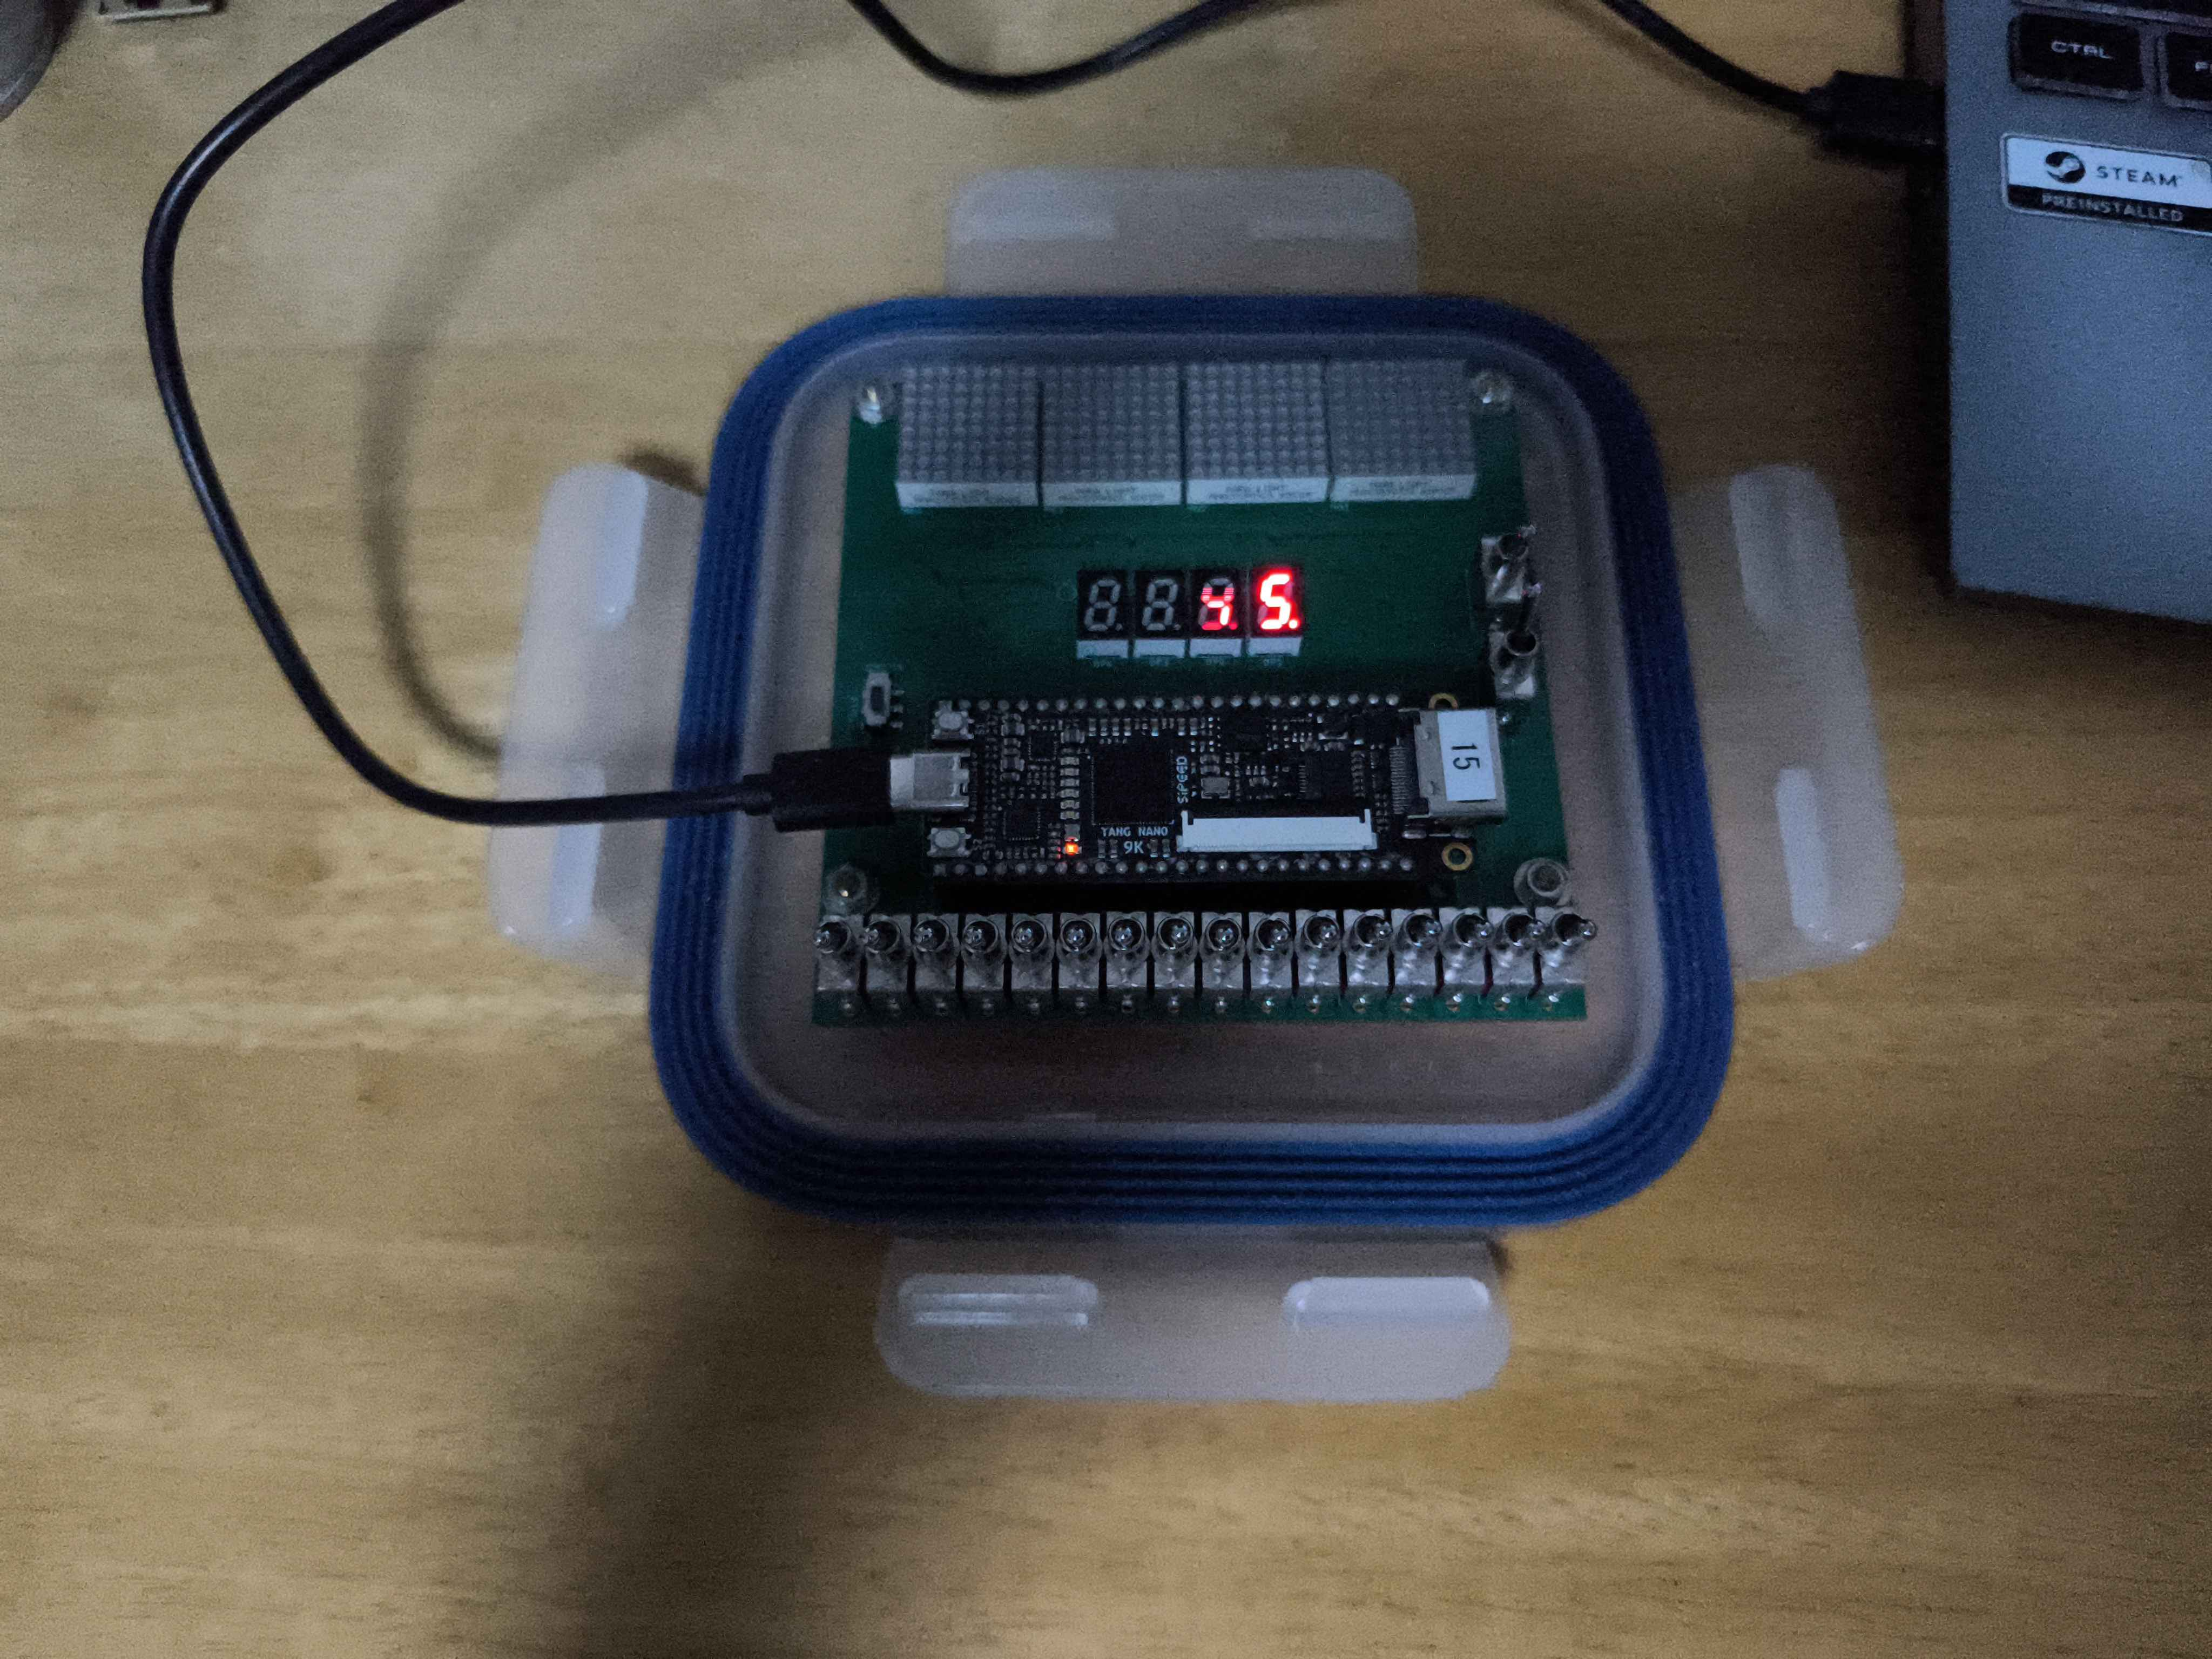
\includegraphics[width=0.6\linewidth]{./image/result3.jpg}
    \caption{FPGAボードの動作確認画像3(露光時間1/2000秒)}
    \label{fig:fpga3}
\end{figure}
\subsection{今後の課題と改善点}
本実験を通じて，いくつかの改善点や今後の課題が明らかになった．

\subsubsection{シミュレーション時間の短縮}
実際の分周比を用いたシミュレーションでは非常に長い時間がかかるため，
今回はクロックを置き換えて検証を行った．
今後は，シミュレーション用のパラメータを設定し，
分周比を可変にできる設計にすることで，
実機と同じ設定でのシミュレーションと，
高速なシミュレーションの両方に対応できるようにすることが望ましい．

\subsubsection{エラー処理の実装}
現在の実装では，カウンタの上限値に達した場合の処理が明確でない．
例えば7桁すべてが9になった後にさらにカウントアップした場合，
オーバーフローが発生して0に戻るが，
この状態を検出して警告を出す機能があると，
より実用的なカウンタになると考えられる．

\subsubsection{消費電力の最適化}
ダイナミック点灯により回路の小型化は実現できたが，
消費電力の観点からの最適化は行っていない．
例えば，表示する桁数が少ない場合に不要な桁の点灯を停止したり，
輝度を調整したりする機能を追加することで，
さらなる省電力化が可能になると考えられる．

\section{結論}
本実験では，順序回路の階層設計手法を用いて10進数カウンタをFPGA上に実装し，
以下の成果を得た．

\begin{enumerate}
    \item 階層設計により，複雑な回路を機能単位のモジュールに分割し，効率的に設計・実装できることを実証した．
    \item Verilog HDLを用いた回路設計とシミュレーションにより，実機での動作確認前にロジックエラーを検出・修正できることを確認した．
    \item ダイナミック点灯を用いた4桁の7セグメントLED表示を実装し，回路の小型化を実現した．
    \item 基本的なカウンタ機能に加えて，加算/減算の切り替え，小数点位置の可変，カウント停止/再開といった拡張機能を実装し，カウンタの汎用性を向上させた．
    \item 同期設計の重要性を理解し，安定した回路動作を実現した．
\end{enumerate}

これらの成果により，FPGAを用いた大規模回路の設計手法と，
HDLによる回路記述の基本を習得することができた．
今後は，本実験で得た知識を基に，
より複雑な順序回路や組み合わせ回路の設計に取り組んでいきたい．

\end{document}